\noindent
\begin{minipage}[t]{0.27\textwidth}
  \vspace*{42pt}
  {\sffamily\footnotesize\raggedright
  Hình 3 biểu diễn đồ thị của hàm số trong Ví dụ 4 và đạo hàm của nó. Chú ý rằng khi $y$ tăng nhanh (gần $-\sqrt[3]{6} \approx -1{,}8$), $y'$ rất lớn. Và khi $y$ tăng chậm, $y'$ gần bằng 0.\par}

  \vspace{8pt}
  \noindent
  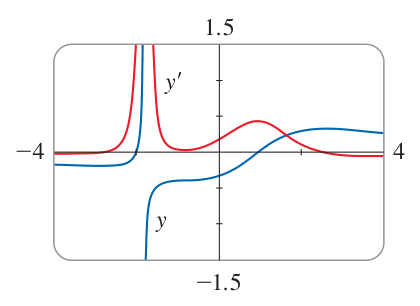
\includegraphics[width=\linewidth]{images/p0223_fig1.png}
  
  \vspace{4pt}
  \noindent{\sffamily\bfseries\footnotesize\color{stewartcyan}HÌNH 3}\par

  \vspace{122pt}
  \noindent
  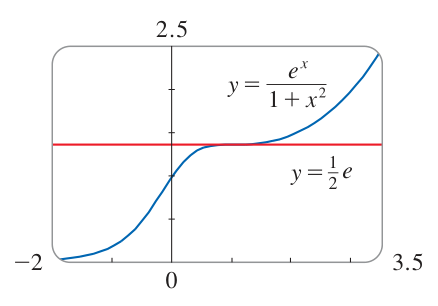
\includegraphics[width=\linewidth]{images/p0223_fig2.png}
  
  \vspace{4pt}
  \noindent{\sffamily\bfseries\footnotesize\color{stewartcyan}HÌNH 4}\par
\end{minipage}%
\hfill
\begin{minipage}[t]{0.69\textwidth}
  \noindent
  Quy tắc thương và các công thức đạo hàm khác cho phép chúng ta tính đạo hàm của bất kỳ hàm phân thức hữu tỉ nào, như ví dụ tiếp theo minh họa.

  \vspace{8pt}
  \noindent
  \textbf{\textsf{\color{stewartcyan}VÍ DỤ 4}}\quad Cho $y = \dfrac{x^2 + x - 2}{x^3 + 6}$. Khi đó
  \begin{align*}
    y' &= \frac{(x^3 + 6)\frac{d}{dx}(x^2 + x - 2) - (x^2 + x - 2)\frac{d}{dx}(x^3 + 6)}{(x^3 + 6)^2} \\[6pt]
       &= \frac{(x^3 + 6)(2x + 1) - (x^2 + x - 2)(3x^2)}{(x^3 + 6)^2} \\[6pt]
       &= \frac{(2x^4 + x^3 + 12x + 6) - (3x^4 + 3x^3 - 6x^2)}{(x^3 + 6)^2} \\[6pt]
       &= \frac{-x^4 - 2x^3 + 6x^2 + 12x + 6}{(x^3 + 6)^2} \tag*{{\color{stewartcyan}\blacksquare}}
  \end{align*}

  \vspace{4pt}
  \noindent
  \textbf{\textsf{\color{stewartcyan}VÍ DỤ 5}}\quad Tìm phương trình tiếp tuyến của đường cong $y = e^x/(1 + x^2)$ tại điểm $(1, \frac{1}{2}e)$.

  \vspace{6pt}
  \noindent
  \textbf{\textsf{\color{stewartcyan}LỜI GIẢI}}\quad Theo Quy tắc thương, ta có
  \begin{align*}
    \frac{dy}{dx} &= \frac{(1 + x^2)\frac{d}{dx}(e^x) - e^x \frac{d}{dx}(1 + x^2)}{(1 + x^2)^2} \\[6pt]
                  &= \frac{(1 + x^2)e^x - e^x(2x)}{(1 + x^2)^2} = \frac{e^x(1 - 2x + x^2)}{(1 + x^2)^2} \\[6pt]
                  &= \frac{e^x(1 - x)^2}{(1 + x^2)^2}
  \end{align*}
  Vậy hệ số góc của tiếp tuyến tại $(1, \frac{1}{2}e)$ là
  \[
    \left.\frac{dy}{dx}\right|_{x=1} = 0
  \]
  Điều này có nghĩa là tiếp tuyến tại $(1, \frac{1}{2}e)$ nằm ngang và phương trình của nó là $y = \frac{1}{2}e$. (Xem Hình 4.) \hfill {\color{stewartcyan}$\blacksquare$}

  \vspace{12pt}
  \noindent
  \textbf{\textsf{\color{stewartgreen}GHI CHÚ}}\quad Đừng sử dụng Quy tắc thương \textit{mỗi khi} bạn nhìn thấy một thương. Đôi khi việc biến đổi thương thức trước để đưa nó về dạng đơn giản hơn cho mục đích tính đạo hàm sẽ dễ dàng hơn nhiều. Chẳng hạn, mặc dù có thể tính đạo hàm của hàm số
  \[
    F(x) = \frac{3x^2 + 2\sqrt{x}}{x}
  \]
  bằng Quy tắc thương, nhưng sẽ thuận tiện hơn rất nhiều nếu thực hiện phép chia trước và viết hàm số dưới dạng
  \[
    F(x) = 3x + 2x^{-1/2}
  \]
  trước khi tính đạo hàm.
\end{minipage}

\vfill
\noindent
{\tiny\color{gray}Copyright 2021 Cengage Learning. All Rights Reserved. May not be copied, scanned, or duplicated, in whole or in part. WCN 02-200-203\par
\noindent Editorial review has deemed that any suppressed content does not materially affect the overall learning experience. Cengage Learning reserves the right to remove additional content at any time if subsequent rights restrictions require it.\par}
